\section{Solids as Interacting Quantum Many-Body Systems}
% HW0 - Practical examples of what you should already know. Go through first 3 chapters of A&M

In this class we will largely discuss the theory of solids. A solid is anything that is rigid, but specifically we will discuss solids as ions arranged in a regular lattice plus electrons.

\begin{figure}[htbp]
    \centering
    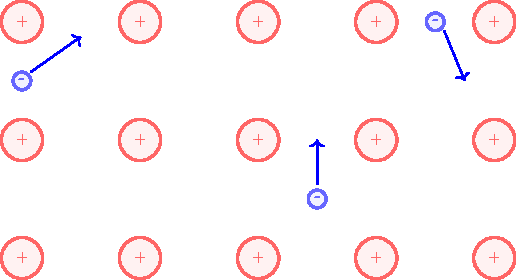
\includegraphics[scale=0.7]{Images/fig-solidcartoon.pdf}
    \caption{A cartoon visualization of a solid, here a square regular lattice with free electrons.}
    \label{fig-solidcartoon}
\end{figure}

\subsection{A Condensed Matter Theory of Everything}
Consider the Hamiltonian:
\begin{equation}
    H = \sum_i \frac{P_i^2}{2M} + \frac{(Ze)^2}{2}\sum_{i, i'}\frac{1}{\abs{\v{R}_i - \v{R}_{i'}}} + \sum_j \frac{p_j^2}{2m} + \frac{e^2}{2}\sum_{j, j'}\frac{1}{\abs{\v{r}_i - \v{r}_{i'}}} - Ze^2\sum_{i, j}\frac{1}{\abs{\v{R}_i - \v{r}_j}}.
\end{equation}
First term is ion KE, second term is ion-ion Coulomb interaction, third term is electron KE, fourth term is electron-electron Coulomb interaction, fifth term is ion-electron Coulomb interaction. This is in principle the theory of everything, which encompasses all that there is need to know in a solid. Note that spin is missing here; we should add two copies of everything (spin up, spin down) and relativistic effects (spin orbit coupling) but for most solids these are relatively small corrections. However, there is a large problem; this is a largely intractable problem. The main problem is that $N$ (the number of electrons in a given solid) is extremely large; $N \sim 10^{23}$. Let's consider some cases of $N$.
\begin{itemize}
    \item $N = 1$ is the hydrogen atom; this has been solved by Schrodinger (and in undergraduate QM) exactly.
    \item $N = 2$ is the Helium atom; already there exists no exact solution. But there are approximate methods that work well (e.g. variational principle for finding the ground state energy)
    \item $N = 1-100$ is the whole of chemistry; there are more sophisticated approximation techniques here.
    \item $N \sim 10^{23}$ is the theory of solids.
\end{itemize}
The key issue of the problem is the size of the corresponding Hilbert space is \emph{enormous}. It's even hard to estimate how large, as position and momentum are continuous. But just to illustrate the size of $\H$ for $N = 10^{23}$, let's consider a simpler setting where we only consider spin and ignore all of the motional degrees of freedom. For spin, there are two states; $\uparrow$ and $\downarrow$ per electron. So the total number of basis states is $2^{N} = 2^{10^{23}} \approx 10^{10^{23}/3}$. There is no computer possible that can store this much information! In fact as an amusing comparison, there are only $3.8 \times 10^{50}$ atoms on Earth, $1.2 \times 10^{57}$ atoms on the sun, and $1.3 \times 10^{79}$ atoms in the visible universe; our brute force method is destined to fail. Our conclusion is that drastic approximations are required in order to make progress in any valid description of solids. And note that they may be drastic, but these approximations turn out to be quite good; there is some simplicity that emerges from what seems to be a hopelessly large and complex Hilbert space. We can achieve a very good understanding of many things; e.g. the physics necessary to construct the device on which this document was written.

\subsection{The Born-Oppenheimer Approximation}
The Born-Oppehnheimer, or adiabatic approximation was originally developed as an approximation method to describe complex molecules; however it applies to our current discussion of solids. It is based on the observation that $M \gg m$ (where $M$ is the ion mass and $m$ the electron mass), namely $\frac{m}{M} \sim 10^{-3}-10^{-5}$. We imagine that in a complicated system of electrons and ions we have equipartition of energy\footnote{Equipartition is a result from classical physics, but it applies suprisingly well.}; because the energy scales of electrons and ions are comparable, the electrons will be moving much faster. Therefore it is possible to decouple the problem of electrons and phonons, by solving the electron motion on a static background of ions. 

One can deduce that $v_{ion} \sim \left(\frac{m}{M}\right)^{3/4}v_F \sim 10^{-2}-10^{-3}v_F$. Also, $v_F \sim 3 \times 10^{6}\si{m/s} \sim 10^{-2}c$ so the physics we consider is non-relativistic (and we can add corrections to the order of 1\%). There are various supposedly intuitive arguments for why we have a power of $3/4$ on $\frac{m}{M}$, but most are not at all obvious or really reasonable; we will derive it after going further into our discussion of solids.

We explore the consequences of $v_{ion} \ll v_F$ for solutions of the Schrodinger equation:
\begin{equation}\label{eq-SE}
    H\psi(\v{r}, \v{R}) = E\psi(\v{r}, \v{R})
\end{equation}
where $\v{r} = \set{\v{r}_j}_j$ and $\v{R} = \set{\v{R}_i}_i$. We make the ansatz:
\begin{equation}
    \psi(\v{r}, \v{R}) = \sum_n \phi_n(\v{R})\psi_{e, n}(\v{r}, \v{R})
\end{equation}
where $\psi_{e, n}$ are solutions to the \emph{electron} problem at fixed ion positions. In other words:
\begin{equation}\label{eq-fixedionansatz}
    \boxed{(T_e + V_{ee} + V_{ei})\psi_{e, n}(\v{r}, \v{R}) = E_{e, n}(\v{R})\psi_{e, n}(\v{r}, \v{R})}
\end{equation}
This in itself is an intractable problem, but it will be useful for our analysis to assume a solution of this form. Let us substitute our ansatz into the SE. We then obtain:
\begin{align*}
    (T_i + T_e + V_{ii} + V_{ee} + V_{ei})\psi = E\psi.
\end{align*} 
We can rewrite this as:
\begin{align*}
    (T_i + V_{ii})\psi + \sum_n \phi_n(T_e + V_{ee} + V_{ei})\psi_{e, n} = E\psi
\end{align*}
But the term in brackets of the sum if the electronic part, so:
\begin{equation}
    (T_i + V_{ii})\psi + \sum_n E_{e, n}(\v{R})\psi_{e, n}(\v{r}, \v{R}) = E\psi
\end{equation}
We can not multiply by $\psi^{*}_{e, m}(\v{r}, \v{R})$ and integrate over $\v{r}$. We then have many simplifications that arise from orthonormality (namely in the second term and the RHS). But the first term on the RHS is nontrivial as $T_i$ contains $\nabla_{\v{R}}$. In any case, we are left with:
\begin{equation}
    \sum_n \int d\v{r}\psi^*_{e, m}(\v{r}, \v{R})T_i \phi_n(\v{R})\psi_{e, n}(\v{r}, \v{R}) + (V_{ii} + E_{e, m}(\v{R}) - E)\phi_M(\v{R}) = 0.
\end{equation}
where we have used the orthonormality of $\psi_{e, n}$ to collapse most of the terms. Let us now analyze the troublesome term. We rewrite this as $\sum_{i}\bra{em}\frac{P_i^2}{2M}\phi_n(\v{R})\ket{en}$. $P_i^2$ is a second derivative, so we end up getting three terms; one term where both derivatives act on $\phi_n$, a term where one acts on $\phi_n$ and the other on $\ket{en}$, and the last where both act on $\ket{en}$. Explicitly, we can write it as:
\begin{equation}\label{eq-problematicterm}
    \sum_{i}\bra{em}\frac{P_i^2}{2M}\phi_n(\v{R})\ket{en} = -\frac{\hbar^2}{2M}\sum_i \int d\v{r}\psi^*_{e, m}(\v{r}, \v{R})\left[(\nabla_{R_i}^2\phi_n(\v{R})) + 2(\nabla_{R_i}\phi_n(\v{R}))\nabla_{R_i} + \phi_n(\v{R})\nabla_{R_i}^2\right]\psi_{e, n}(\v{r}, \v{R}).
\end{equation}
The first term can be evaluated (as before) using orthonomality. The other two are not as convenient, but in the B-O approximation we may neglect the other two terms (and we will discuss shortly why this is a good idea).

We obtain the following equation:
\begin{equation}\label{eq-phononeq}
    \boxed{[T_i + V_{ii} + E_{e, n}(\v{R})]\phi_n(\v{R}) = E_n\phi_n(\v{R})}
\end{equation}

Note we can solve Eq. \eqref{eq-fixedionansatz} assuming the ions are static/in fixed positions. From there we obtain $E_{e, n}(\v{R})$ which allows us to solve Eq. \eqref{eq-phononeq} (which is known as a phonon equation), which allows us to obtain $E_n$ and $\phi_n(\v{R})$, which gives us the solution of the whole problem. We have decoupled one very complex problem into two connected but separately solvable equations. $E_{e, n}(\v{R})$ is called the effective ionic potential; without it a crystal would blow apart (via repulsive interaction), but it holds things together. 

As a last step, we must still demonstrate that the two neglected terms in \eqref{eq-problematicterm} make negligible contributions. One can show that:
\begin{enumerate}
    \item The first term is order $\left(\frac{m}{M}\right)^{1/2}\e_F$.
    \item The second term is order $\left(\frac{m}{M}\right)^{3/4}\e_F$.
    \item The third term is order $\left(\frac{m}{M}\right)\e_F$.
\end{enumerate}

However these estimates are for now opaque; we will confirm them later by further analysis. For now though, we recall that $\frac{m}{M} \sim 10^{-3}-10^{-5}$ so the second/third terms tend to be at least an order of magnitude smaller than the first (and can be neglected to first order). However, some important properties of crystalline solids are actually derived from these terms. For example if we analyze how electron motion couples to lattice vibration, then we have to start to worry about them. Additionally, the terms also contribute to resistivity of metals (phonon-electron scattering, especially important at high temperatures; why resistivity drops at lower temps)

So to start, we will study the electron and lattice degrees of freedom separately, but as we go further into our study we will have to revisit these coupling terms. Next week,